% MSc dissertation example file, February 2022
%
% Leave one of the documentclass lines uncommented to match your degree.
% You may remove the logo option if it causes problems.
% Do not change any other options.
% \documentclass[logo,msc,adi]{infthesis}     % Adv Design Inf
% \documentclass[logo,msc,ai]{infthesis}      % AI
% \documentclass[logo,msc,cogsci]{infthesis}  % Cognitive Sci
% \documentclass[logo,msc,cs]{infthesis}      % Computer Sci
% \documentclass[logo,msc,cyber]{infthesis}   % Cyber Sec
% \documentclass[logo,msc,datasci]{infthesis} % Data Sci
% \documentclass[logo,msc,di]{infthesis}      % Design Inf
% \documentclass[logo,msc,dsti]{infthesis}    % Data Sci TI
% \documentclass[logo,msc,inf]{infthesis}     % Informatics
\documentclass[logo,msc]{infthesis}           % degree unspecified, do not change except to add your degree
%%%%%%%%%%%%%%%%%%%%%%%%
% Understand any problems and seek approval before assuming it's ok to remove ugcheck.
\usepackage{msccheck}

% Include any packages you need below, but don't include any that change the page
% layout or style of the dissertation. By including the ugcheck package above,
% you should catch most accidental changes of page layout though.

\usepackage{microtype} % recommended, but you can remove if it causes problems

\begin{document}
\begin{preliminary}

\title{Design and Implementation of a Resource-based Checklist Generation Tool}

\author{Watcharin 'Aun' Sirinaovakul}

\date{\today}

\abstract{
% This skeleton demonstrates how to use the \texttt{infthesis} style for
% MSc dissertations in the School of Informatics. It also emphasises the
% page limit and associated style restrictions for Informatics dissertations
% with course code \texttt{INFR11077}. If your degree has a different project
% course code, then it is likely to have different formatting rules.
% The file \texttt{skeleton.tex} generates this document and should be used as a
% starting point for your thesis. Replace this abstract text with a concise
% summary of your report.

% what I did, evaluation
}

\maketitle

\newenvironment{ethics}
   {\begin{frontenv}{Research Ethics Approval}{\LARGE}}
   {\end{frontenv}\newpage}

\begin{ethics}
% IF ETHICS APPROVAL WAS REQUIRED:
This project obtained approval from the Informatics Research Ethics committee.\\
Ethics application number: 486463\\
Date when approval was obtained: 2022-06-30

\standarddeclaration
\end{ethics}


\begin{acknowledgements}
Any acknowledgements go here.
\end{acknowledgements}


\tableofcontents
\end{preliminary}


\chapter{Introduction}
% objective, users, benefits, scope of work, relevant works, previous works, future works, project background, techniques

% The preliminary material of your report should contain:
% \begin{itemize}
% \item
% The title page.
% \item
% An abstract page.
% \item
% Declaration of ethics and own work.
% \item
% Optionally an acknowledgements page.
% \item
% The table of contents.
% \end{itemize}

% As in this example \texttt{skeleton.tex}, the above material should be
% included between:
% \begin{verbatim}
% \begin{preliminary}
%     ...
% \end{preliminary}
% \end{verbatim}
% This style file uses roman numeral page numbers for the preliminary material.

% The main content of the dissertation, starting with the first chapter,
% starts with page~1. \emph{\textbf{The main content must not go beyond page~40.}}

% The report then contains a bibliography and any appendices, which may go beyond
% page~40. The appendices are only for any supporting material that's important to
% go on record. However, you cannot assume markers of dissertations will read them.

% You may not change the dissertation format (e.g., reduce the font size, change
% the margins, or reduce the line spacing from the default 1.5 spacing). Be
% careful if you copy-paste packages into your document preamble from elsewhere.
% Some \LaTeX{} packages, such as \texttt{fullpage} or \texttt{savetrees}, change
% the margins of your document. Do not include them!

% Over-length or incorrectly-formatted dissertations will not be accepted and you
% would have to modify your dissertation and resubmit. You cannot assume we will
% check your submission before the final deadline and if it requires resubmission
% after the deadline to conform to the page and style requirements you will be
% subject to the usual late penalties based on your final submission time.

% \section{Using Sections}

% Divide your chapters into sub-parts as appropriate.

% \section{Citations}

% Citations (such as \cite{P1} or \cite{P2}) can be generated using
% \texttt{BibTeX}. For more advanced usage, we recommend using the \texttt{natbib}
% package or the newer \texttt{biblatex} system.

% These examples use a numerical citation style. You may use any consistent
% reference style that you prefer, including ``(Author, Year)'' citations.


% objective, users, benefits, scope of work, relevant works, previous works, future works, project background, techniques

-Probably what a workflow is-

Business process management (BPM) tools are software to help design, automate, and manage systematic workflows for various business areas. The ease with which repetitive task automation can be implemented using BPM tools is one of its primary benefits. That is because it requires no prior coding experience to develop a workflow in BPM tools. However, the tools are sufficiently customisable for a more experienced user to create a more complex workflow.

% WorkflowFM \cite{papapanagiotou2017workflowfm} is a BPM tool developed and maintained by a research team at the University of Edinburgh that allows people in various industries to build their automated workflows from scratch. What distinguishes WorkflowFM from other competitors is that the models are based on the data structure of the input and output of each task. This further reduces the complexity when generating codes since the system can rely on the structure of the resources rather than the arbitrary input and output defined by users. Moreover, WorkflowFM can generate code required for the control flow automatically. Despite the advantages provided by WorkflowFM, it is still in a very early stage with limited features.

WorkflowFM \cite{papapanagiotou2017workflowfm} is a BPM tool developed by a research team at the University of Edinburgh.
% WorkflowFM's main goal is to help create workflows strictly to the data models within the system. That means each process needs to strictly follow the data models provided within the system and no arbitrary information are allowed.
The objective of WorkflowFM is to assist in developing workflows that rigorously adhere to the system's data models. This means that no random information is permitted and that each process must strictly follow to the data models supplied within the system.
% Compared to other competitors which do not rigorously conform to the data models, WorkflowFM is easier to ge
Nevertheless, WorkflowFM is still in a very early stage with limited features.

-Probably what a checklist is and why it is important-

-What I am going to do in this project-

-What scope of the project I am looking to do-

-What end results of the project should look like-


\chapter{Background}

\section{Business Process Management Tools}
% Business Process Management (BPM) is a methodology that involves designing, controlling, and analysing business processes to support organisations \cite{bpmdefinition}. 
% BPM's stages is defined differently depending on references \cite{bpmlifecycles, bpmlifecycles2, bpmlifecycles3}; however, it generally consists of at least four stages: i) analysing; ii) modeling; iii) implementing; iv) executing.
% As for BPM tools, they are software solutions that support organisations in all stages of BPM with little to no coding knowledge. As a consequence, BPM tools are widely used in various industries.
Business Process Management (BPM) is a discipline that assist business analysts in planning, monitoring and analysing processes to support businesses \cite{bpmdefinition}. BPM methodologies could generally be separated into four different stages: i) analysing; ii) modelling; iii) implementing; iv) execution \cite{bpmlifecycles, bpmlifecycles3, bpmlifecycles2}.
BPM tools are software that makes use of this concept in assisting business analysts model processes with little to no coding knowledge to help businesses build automatic streamlining and reduce wastes in manufacturing processes 
\cite{bpmtoolwaste}.

One of the advantages of using BPM tools is the orchestration between systems, humans, and workflows \cite{bpmstrength}.
This improves the efficiency of business processes in organisations by formalising processing into structured methods that can be monitored, analysed, and automated easily \cite{bpmbenefits}.
BPM tools use checklists that are integrated as part of a workflow to efficiently coordinate humans and workflows by integrating inputs into the workflow. For example, Bizagi \cite{bizagi}, one of the widely known BPM tools, can construct checklists or forms within its automated workflows and connect the checklists to the following processes using the shared database technique. Nintex \cite{nintext} is another widely used BPM tool that also adopts the idea of checklist and implements it in their environment. This provides a variety of options for workflow users to interact with the workflows in the system.


\section{WorkflowFM}
\label{background:workflowfm}

WorkflowFM \cite{papapanagiotou2017workflowfm} is a logic-based BPM tool developed by researchers from the University of Edinburgh. Being a logic-based framework means all the inputs, outputs, and processes follow the validation defined by the framework.
Each process is validated by WorkflowFM to ensure that it is logically valid, correctly matched with neighbour processes, and functional as a workflow.
As a logic-based BPM tool, WorkflowFM differs from other frameworks in that processes are defined based on inputs and outputs with preconditions, as opposed to most BPM tools which accept any Business Process Model and Notation (BPMN) \cite{bpmn} format when creating a workflow. Moreover, it requires the inputs and outputs in each process to match when connected to other processes.
% Additionally, WorkflowFM requires defining data models for each input and output
% only require a XML pattern to create a workflow as XML is the standardised format for BPM tools.
% unlike various BPM tools which follows the XML Process Definition Language (XPDL), the standard format for interchanging process definitions between different BPM tools \cite{xmlpdl}.



WorkflowFM's system architecture, as shown in Figure \ref{fig:workflowfm-system}, includes two main groups of components: modelling and execution. Modelling is the part that allows users to create workflows, and execution is the component that operates deployed workflows in the system. This project aims to build a checklist generation tool as an extension to the execution engine to help generate checklists in WorkflowFM and allow people to perform tasks through checklists for executing workflow processes.


% , which contains two components: composer and reasoner. The composer component assists users in creating workflows, while the reasoner validates that the workflows produced by the composer adhere to the defined inputs and outputs.
% On the other hand, m and contains three components: execution engine, simulation engine, and dashboard.
% The checklist generation will be placing in the execution group as an extension to the execution engine.

% WorkflowFM's system architecture, as shown in Figure \ref{fig:workflowfm-system}, includes two main groups of components: modelling and execution. Modelling is the part that allows users to create workflows, which contains two components: composer and reasoner. The composer component assists users in creating workflows, and the reasoner validates that the workflows produced by the composer adhere to the defined inputs and outputs.
% On the other hand, execution is the component that operates deployed workflows in the system. Execution contains execution engine, simulation engine, and dashboard.
% This project aimed to build was a checklist generation tool that connects with the execution engine as an extension to generate checklists and allow people to perform tasks for executing workflow processes.
% The execution engine and the simulation engine are integrated with each other and directly connect to the dashboard to visualise deployed workflows. Furthermore, the checklist generation connects with the execution engine as an extension to generate checklists and allow people to perform tasks for workflows.
% Unlike Bizagi or Nintex, WorkflowFM is a logic-based framework which 

\begin{figure}
    \centering
    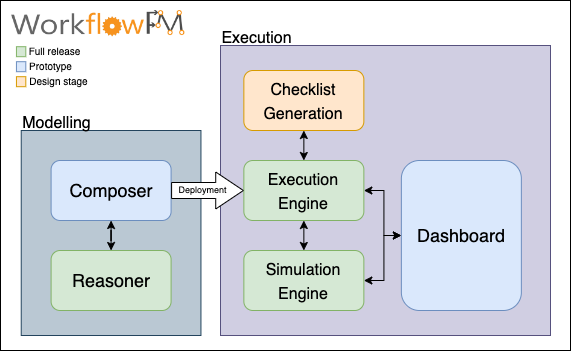
\includegraphics[width=0.7\textwidth]{overleaf/images/workflowfm-system.png}
    \caption{WorkflowFM's System Architecture}
    \label{fig:workflowfm-system}
\end{figure}

As of now, WorkflowFM has been used in the healthcare and manufacturing domains. With the expanding usage of the framework, the checklist generation becomes more desirable for people in the industries. However, checklist generation is still at the design stage and has not been implemented. That is why this project focuses on implementing a prototype of the checklist generation.

% As of now, WorkflowFM has been used in the healthcare domain \cite{papapanagiotou2014formal} and expanding to the manufacturing domain. With in increasing of ..., this is why a checklist generation tool is needed in WorkflowFM.

\section{WorkflowFM's Process}
\label{background:input_output}

Each process in WorkflowFM contains a unique name and a group of inputs and a group of outputs. Each input and output is represented as a node that can be either atomic, parallel, or optional. 
An atomic is a representation of an entity \cite{entity} that exists in the system,
a parallel is a representation of selecting every children node,
and an optional is a representation of selecting one among all the children nodes.
Combining the nodes together would form a tree of nodes, which a leaf node must be an atomic.

For example, according to the running example in Section \ref{running_example}, the process's name is \verb!Payment Process!, the input contains an optional node that can be either an order (\verb!order!) or an order with discounts (\verb!order with discounts!), and the output contains a parallel node of the billing address (\verb!billing address!) and an optional node that can be either PayPal (\verb!paypal!) or Debit/Credit card (\verb!debit/credit card!). A visualisation of the inputs and outputs can be visualised in Figure \ref{fig:type_nodes_example}.

\begin{figure}[ht!]
    \centering
    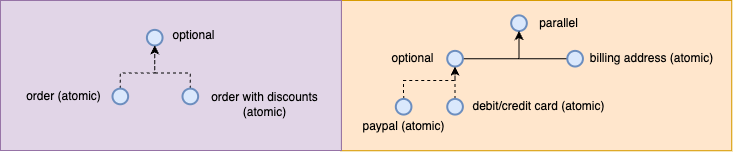
\includegraphics[width=\textwidth]{overleaf/images/type_nodes_example.png}
    \caption{Inputs (Left) and Outputs (Right) Visualisation}
    \label{fig:type_nodes_example}
\end{figure}


% A JSON-based format \cite{json} is used in WorkflowFM to specify processes.
% The JSON format used in WorkflowFM includes several fields that are used in different parts of the system, which can be seen in Figure \ref{fig:workflowfm_json}.
% However, the name, input and output of each process are the only requirements to generate a resource-based checklist template.
% % Each model consists of \verb!type!, \verb!name!, and \verb!args!. There are only three types in \verb!type!: \verb!var!, \verb!plus!, and \verb!times!. 

% \begin{figure}[ht!]
%     \centering
%     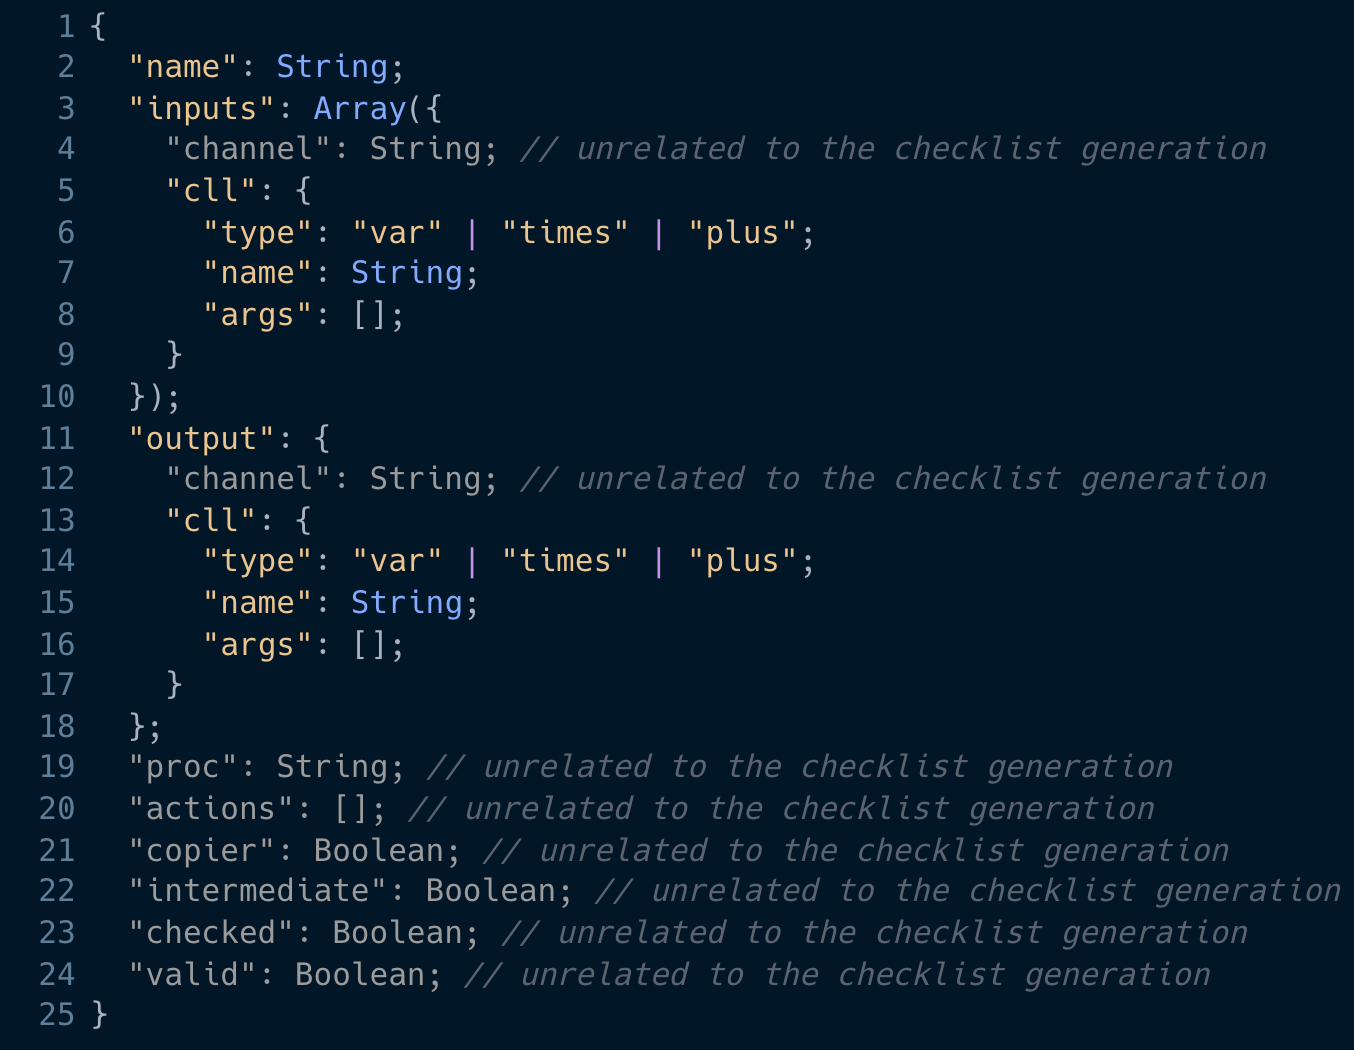
\includegraphics[width=0.75\textwidth]{overleaf/images/workflowfm_json.png}
%     \caption{WorkflowFM's Process JSON}
%     \label{fig:workflowfm_json}
% \end{figure}


% Each input and output node can only be in one of the three types including \verb!var!, \verb!times!, and \verb!plus!.
% A \verb!var! node is a terminal node. That means a \verb!var! node must have no child. Being a \verb!var! node indicates that that specific node is a data model that the process can refer to.
% On the other hand, \verb!times! and \verb!plus! nodes are not data models on its own and must contain child nodes inside it. The child nodes can either be one of the three types recursively, but at terminal nodes, they must be the \verb!var! type.
% \verb!times! and \verb!plus! nodes are different on how they combine the children. \verb!times! merges all the children together as one large data model, while \verb!plus! only selects one of its children to be the data model representing that node.

% All child nodes under \verb!times! are required to exist as the data model representing that node, while only one of the children under \verb!plus! is the representative data model. 

% but they must contain nodes as their children. The difference between \verb!times! and \verb!plus! is all child nodes in a \verb!times! node are compulsory inputs or outputs, while a \verb!plus! node needs only one of the child nodes to be an input or output.

% A process contains nodes from both input and output sides. A node is a representation between three things: a data model, a times operator, and a plus operator. A data model will be referred as the \verb!var! type. A times operator and a plus operator will be referred as \verb!times! and \verb!plus! accordingly. Both \verb!times! and \verb!plus! nodes must contain children since they are not data models. Furthermore, their children can either be \verb!var!, \verb!times!, and \verb!plus!. However, if a child node is either \verb!times! or \verb!plus!, it needs to recursively continue having children. A \verb!var! child, however, contains no children and acts as a terminal node. \verb!times! and \verb!plus! are different on how they operate. \verb!times! combines the children together as one large data model, while \verb!plus! only selects one of its children to be the data model representing that node.

% The input and output of a process are represented as nodes. A node can either be an atomic entity (\verb!var!) \cite{entity} or an operator (\verb!times! or \verb!plus!).
% An atomic entity represents an entity in the system's database.
% An operation which combines multiple nodes is called a times operator, while which selects an entity between a group of nodes is called a plus operator.
% Combining both entities and operators would form into a tree of nodes, which a leaf node of this tree must be an entity.

% For example, in Figure \ref{fig:process_flows} | which has the JSON format provided in Appendix \ref{appendix:fig:example_json}, this is a payment process that receives \verb!orders! and \verb!payment_method! as the input and returns \verb!order_receipt! and either \verb!credit_card_receipt! or \verb!change! as the output depending on what \verb!payment_method! coming in.
% All five of them are terminal nodes and data models of this process. On the input part, both \verb!orders! and \verb!payment_method! are connected to a \verb!times! node indicating that both data models are compulsory. Meanwhile, \verb!credit_card_receipt! and \verb!change! are connected to a \verb!plus! node indicating either one between them can be selected as the representing data model; however, not both. On top of that, the \verb!plus! node is connected to a \verb!times! node along with \verb!order_receipt! indicating both of them are compulsory.

% Ultimately, the input of this payment process is ``\verb!orders! and \verb!payment_method!"; and the output of this payment process is either ``\verb!order_receipt! and \verb!change!" or ``\verb!order_receipt! and \verb!credit_card_receipt!".

% the input node is a \verb!plus! and contains two children: \verb!input_var_node_1! and \verb!input_times_node!. Moreover, one of the children is a \verb!times! and contains two children: \verb!input_var_node_2! and \verb!input_var_node_3!. Ultimately, the input of this process can be either:

% \begin{itemize}
%     \item \verb!input_var_node_1! \vspace{-8px}
%     \item (\verb!input_var_node_2!, \verb!input_var_node_3!)
% \end{itemize}

% The output of the process is less complex in comparison to the input.
% The output node is a \verb!times! and has only two \verb!var! children. This makes (\verb!output_var_node_1!, \verb!output_var_node_2!) as the output of this process.

% That means either \verb!input_var_node_1! or \verb!input_var_node_2! can be the input data model of the process. Meanwhile, the output node is \verb!times! and also contains two children. In contrast to \verb!plus!, \verb!output_var_node_1! and \verb!output_var_node_2! are the output data models of the process.

% \begin{figure}[ht!]
%     \centering
%     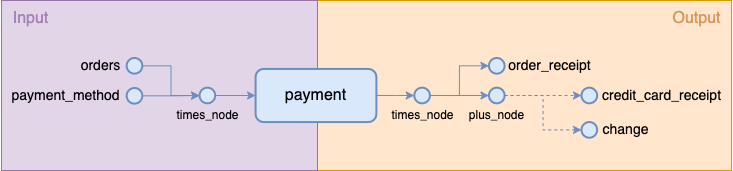
\includegraphics[width=\textwidth]{overleaf/images/process_flows.png}
%     \caption{Example Process}
%     \label{fig:process_flows}
% \end{figure}

\section{Generation of structured checklists from formal \\resource-based workflow models}
\label{background:chens_design}
% This is an MSc project from the previous year written by Yefei Chen \cite{checklistdesign}. Chen has designed the user interface for WorkflowFM's checklist generation tool as well as solved some of the theoretical challenges in the design, such as function-flow chart and data model design. Chen's design consists of six features: i) main page; ii) canvas; iii) edit checklist dependencies; iv) process checklist; v) finished checklist; vi) design of checklist. In the end, the system usability scale questionnaire (SUS) score was mediocre, with a score of 56.5. However, Chen discussed the design weaknesses and provided an analysis of them. Consequently, the results are extremely important since we could continue improving the design based on the analysis.

A design of a resource-based checklist generator has been proposed in Yefei Chen's MSc dissertation \cite{checklistdesign}.
Chen's design is based on the fact that WorkflowFM contains all the data models of the workflow processes in the system and utilises this fact by allowing the checklist generation tool being able to link dependencies with the checklist, which will be further explained in Section \ref{background:dependencies}. This is the feature that we adopted into our project.

Although our project was building on top of Chen's design, Chen's design could not be used to 


\section{Dependencies}

\section{Data Models}


% The design consists of four user interfaces with functionalities on each screen as follow:

% \begin{itemize}
%     \item \textbf{Main Page} is the landing screen of the checklist generator. It can be divided into three sections: \verb!Start A Checklist!, \verb!In Progress!, and \verb!Finished!. The \verb!Start A Checklist! section will bring the user to Canvas screen to create a template. The \verb!In Progress! section is the section that contains all the checklists that has already been started, but not yet finished. And lastly, the \verb!Finished! section contains all the finished checklists.
%     \item \textbf{Canvas} is the building templates screen. It allows users to custom the title, question names, types, and other things in checklists.
%     \item \textbf{Edit Checklist Dependencies} is the screen to manage dependencies in a template. Once a template has been created in Canvas, the designer sometimes needs to adjust dependencies between the input and output. That is to allow the system to create connections between components.
%     \item \textbf{Process Checklist} is the screen of a finished template. It displays the information according to the designed template in Canvas. A finished template, or checklist, in this screen will be used to perform tasks for workflow processes in WorkflowFM.
% \end{itemize}



\chapter{Methodology}
% overall design, architectural design, interface design, database design
% implementation - frontend (main, canvas, checklist) and backend (template creation, template storing, 3, 4)
% user diagram
To accomplish the objectives of this project, we separated them into major milestones and had a weekly meeting with the supervisor to update our progress and see how the schedule went according to the initial plan. In the end, we ended up having four different stages to develop this project: design, implementation, testing, and evaluation.

\section{Design}
Before the design stage, we started gathering and analysing requirements from multiple sources including literature reviews \cite{checklistdesign, papapanagiotou2017workflowfm}, interactive discussion with the product owner|who happened to be my supervisor, and researching upon related tools and projects such as Bizagi \cite{bizagi}, Google Forms \cite{googleforms}, and Microsoft Forms \cite{msforms}.

After we understood the requirements, we began designing the overall system interaction and how the data should enter and exit our system. This includes designing the overall system diagram, the functionalities, software's structure, the interfaces, the use case diagram, the sequence diagrams, and the database.

% the user flow diagram, the diagram flow of the system interaction, checklist template's data models, the use case diagram, the sequence diagrams, the interface design, and the database structure.

\section{Implementation}
In this stage, we built the prototype based on the designs we made. This stage was separated into three major components: frontend, backend, and naive suggestion. The frontend and backend were developed concurrently, and the naive suggestion was added as an additional feature after the other two. Furthermore, we tested the prototype upon more complex processes to support various types of inputs and outputs that might come into the system in the real-world case.
% Furthermore, we decided on the technologies used for this project at this stage.

% \subsection{Testing}
% The testing stage is where the prototype is tested on more complex processes with variety types of inputs and outputs. After performing, we analysed the results and adjusted the prototype on things that needed to be improved.


\section{Evaluation}
At this stage, we conducted a user evaluation in which participants completed two similar tasks with instructions creating checklist templates with and without naive suggestions and another task without instructions. After performing tasks, participants were asked to provide scores on the functionality and usability of the prototype on a scale of 1 to 5.

The usability scores were used to calculate the System Usability Scale (SUS) score \cite{susscores} to evaluate how good the prototype was. Additionally, the results from each task were recorded anonymously and used to compute the precision, recall, and accuracy scores \cite{rocanalysis} on the user performance.


\chapter{Evaluation}
% results
\section{Test Scenario}

\section{Questionnaire}


\section{Unit Testing}


\chapter{Conclusions}
% what the work was, what we did, how we evaluated, what the results were, recommendation for future works
The body of your dissertation, before the references and any appendices,
\emph{must} finish by page~40. The introduction, after preliminary material,
should have started on page~1.

You may not change the dissertation format (e.g., reduce the font size, change
the margins, or reduce the line spacing from the default 1.5 spacing). Be
careful if you copy-paste packages into your document preamble from elsewhere.
Some \LaTeX{} packages, such as \texttt{fullpage} or \texttt{savetrees}, change
the margins of your document. Do not include them!

Over-length or incorrectly-formatted dissertations will not be accepted and you
would have to modify your dissertation and resubmit. You cannot assume we will
check your submission before the final deadline and if it requires resubmission
after the deadline to conform to the page and style requirements you will be
subject to the usual late penalties based on your final submission time.

Future Work blah blah
% workflow user side, security, authentication, authorisation, integration with workflowFM, doing more facility features


\bibliographystyle{plain}
\bibliography{main}


% You may delete everything from \appendix up to \end{document} if you don't need it.
\appendix

\chapter{Participants' information sheet}
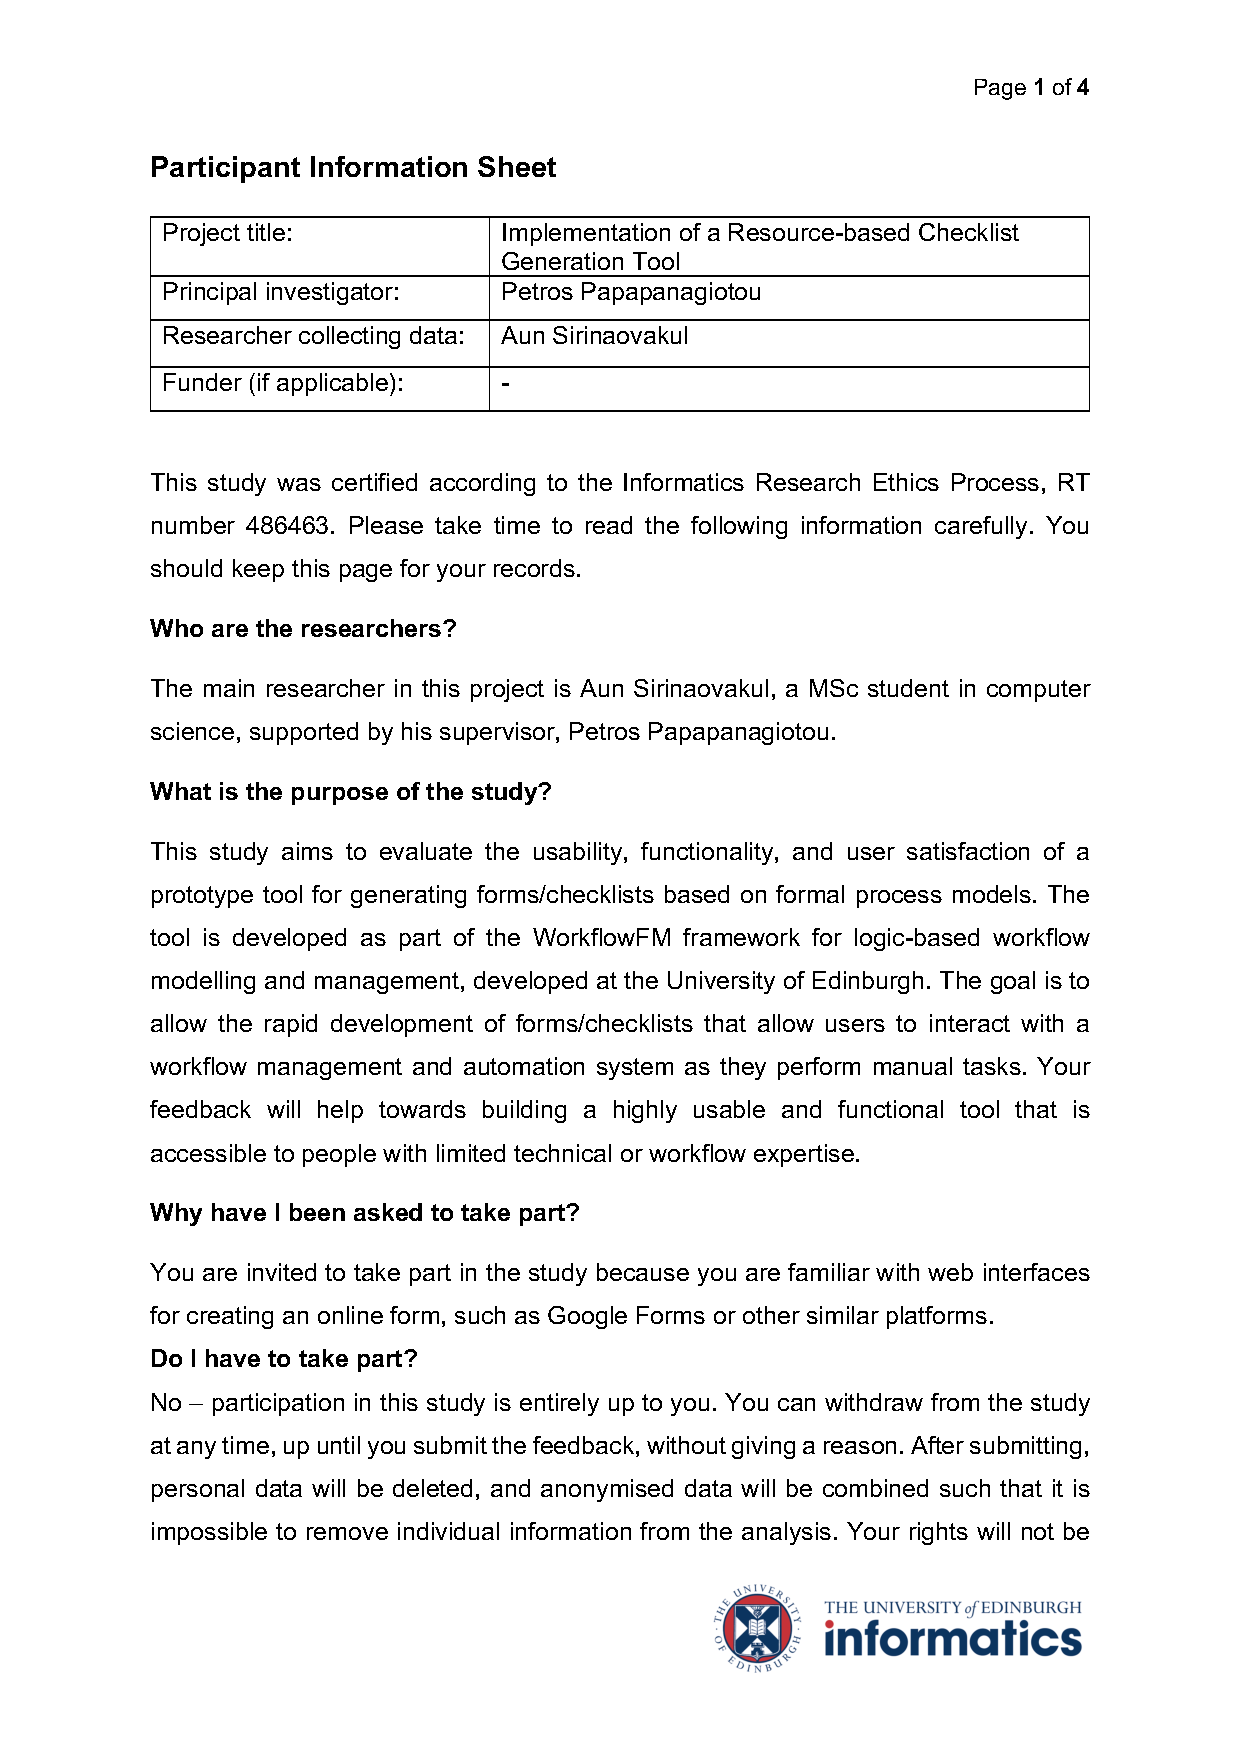
\includepdf[pages=-]{./pdf/PIS.pdf}

\chapter{Participants' consent form}
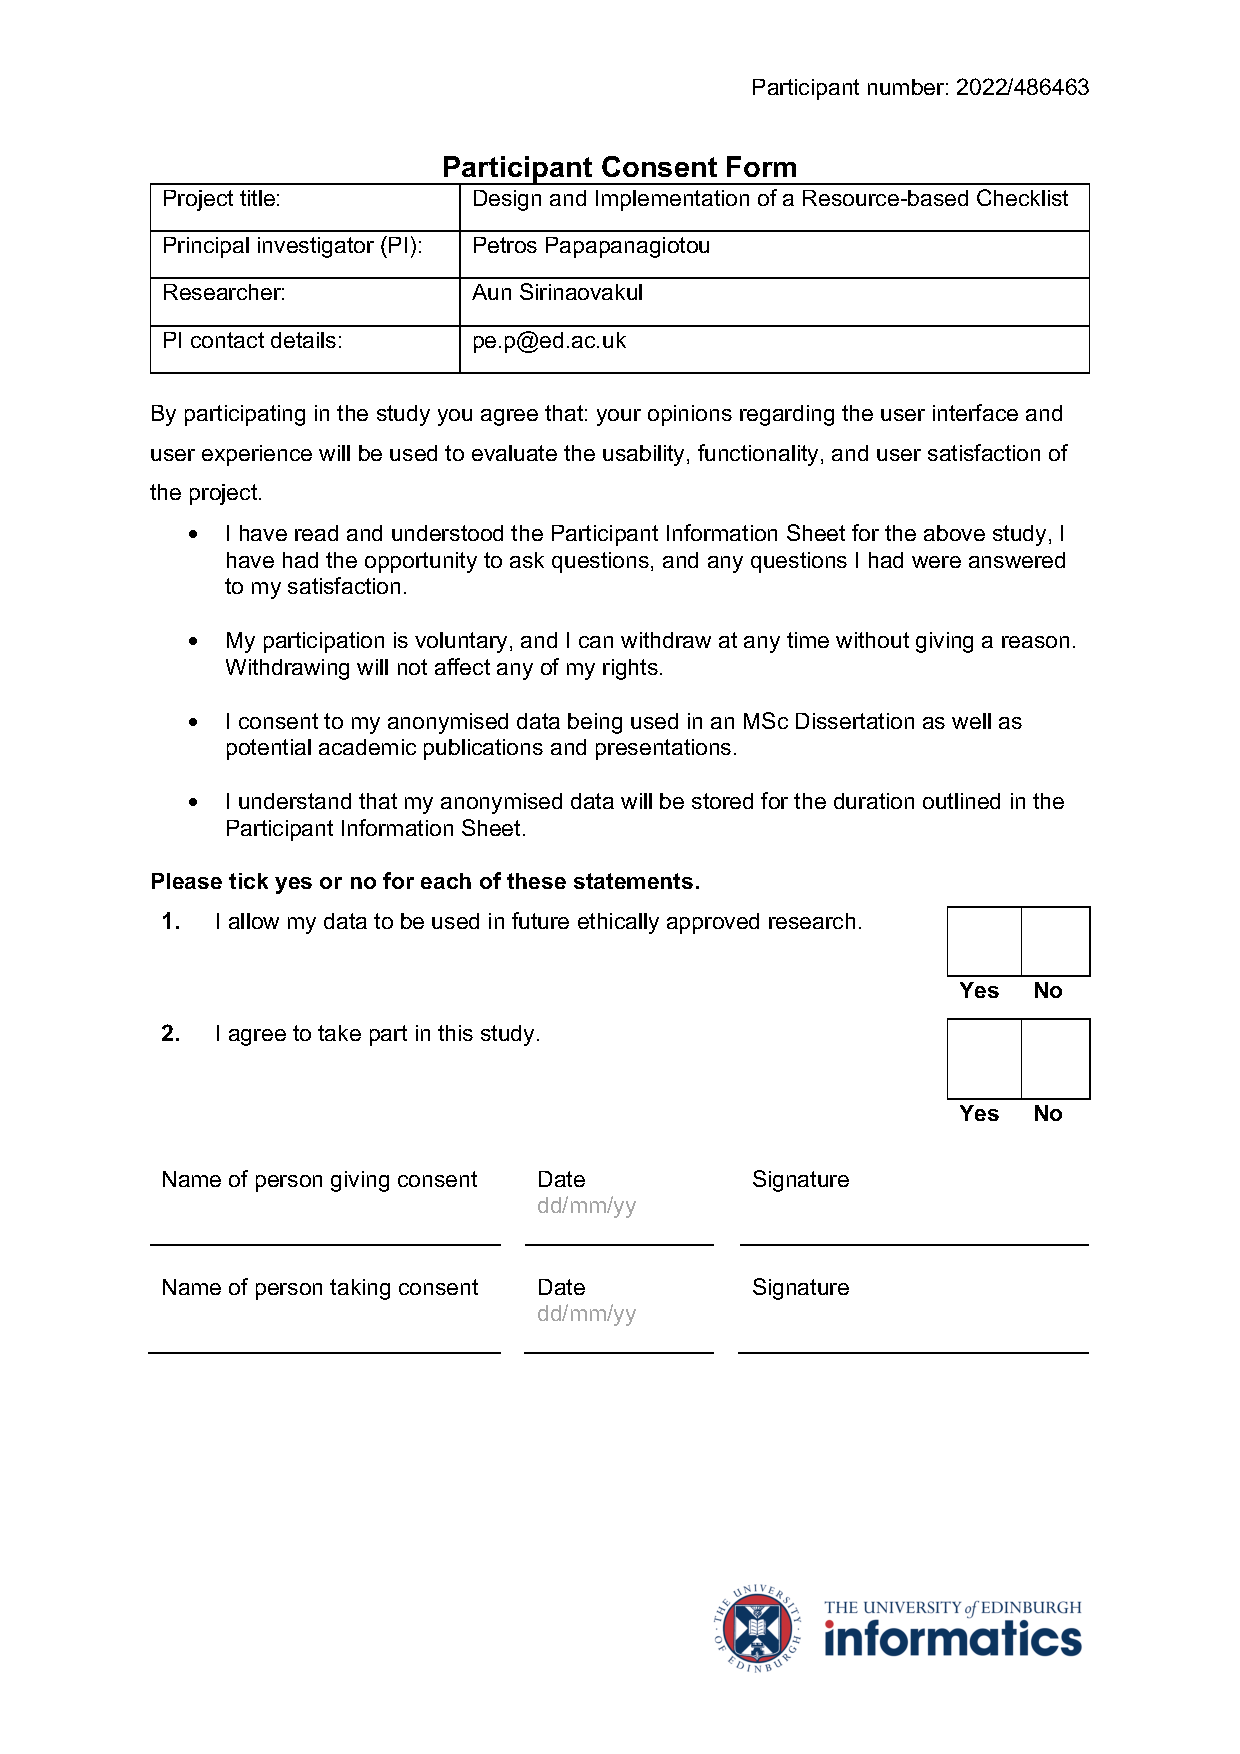
\includepdf[pages=-]{./pdf/Consent Form.pdf}

\chapter{Tasks}

\chapter{Questionaire}


\end{document}
